\begin{table}[htbp]
\centering
\begin{threeparttable}[b]
\caption{本文开发的联邦学习仿真系统集成的数据集}
\label{tab:datasets}
\begin{tabular}{|c|c|c|c|c|}
\hlineB{3.5}
数据集名称 & 规模 & 默认节点数目 & 任务 & 样本类型 \\
\hline \hline
MNIST\tnote{$\ast\dagger$} & 70000 & 1000 & 图像分类 & $28\times 28$的单通道灰度图像 \\
EMNIST\tnote{$\ast$} & 749068 & 3400 & 图像分类 & $28\times 28$的单通道灰度图像 \\
CIFAR10/100\tnote{$\dagger$} & 60000 & 500 & 图像分类 & $32\times 32$的RGB~3通道图像 \\
Shakespeare & 18424 & 715 & 下一字符预测 & 文本 \\
Sent140 & 40783 & 715 & 文本情感分类 & 文本 \\
Synthetic($\alpha, \beta$)\tnote{$\ddagger$} & N/A & N/A & 分类 & 随机生成的高维向量 \\
\hlineB{3.5}
\end{tabular}
\begin{tablenotes}
\item[$\ast$] {\smaller 这两个数据集还有经过筛选\cite{sahu2018fedprox}的规模更小的数据子集,也被本文实现的联邦学习仿真系统\texttt{fl-sim}所包含。}
\item[$\dagger$] {\smaller 这两个数据集还有经过特殊处理,用于研究联邦聚类学习\cite{Ghosh_2022_cfl}的变体,也被本文实现的联邦学习仿真系统\texttt{fl-sim}所包含。}
\item[$\ddagger$] {\smaller 参数$\alpha, \beta$是两个独立的均值为$0$的正态分布的标准差,用于模拟节点内以及节点间的数据分布差异。}
\end{tablenotes}
\end{threeparttable}
\end{table}

MNIST数据集\cite{Lecun_1998_mnist}由手写的阿拉伯数字的图片构成,每张图片是$28\times 28$个像素点组成的灰度图片。图\ref{fig:mnist_random_grid_view}是从MNIST数据集中随机抽取$8\times 16$张图片组成的网格图。MNIST是非常经典的机器学习数据集,经常用作测试机器学习模型,特别是深度学习模型分类效果的基准数据集。尽管随着深度学习的发展,。。。。

\begin{figure}
\centering
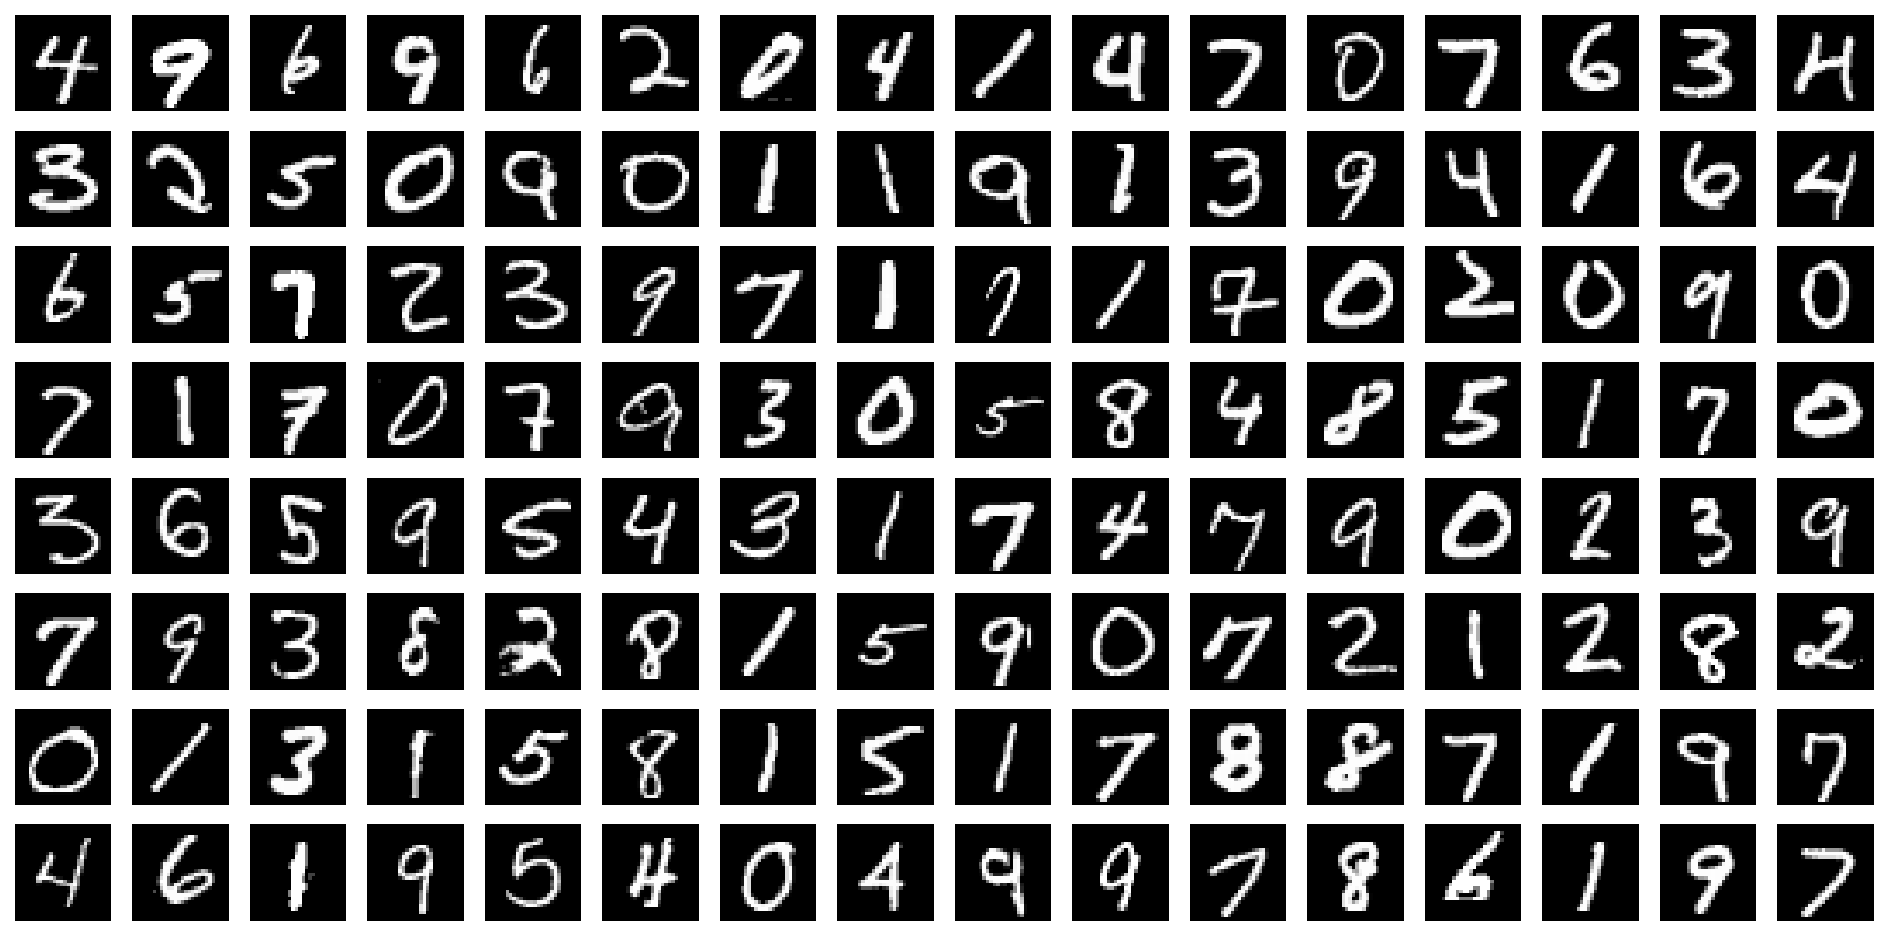
\includegraphics[width=\textwidth]{figures/mnist_random_grid_view.pdf}
\caption{MNIST数据集随机选取的$8\times 16$个样本构成的网格图}
\label{fig:mnist_random_grid_view}
\end{figure}

CIFAR10/100\cite{cifar}

\begin{figure}
\centering
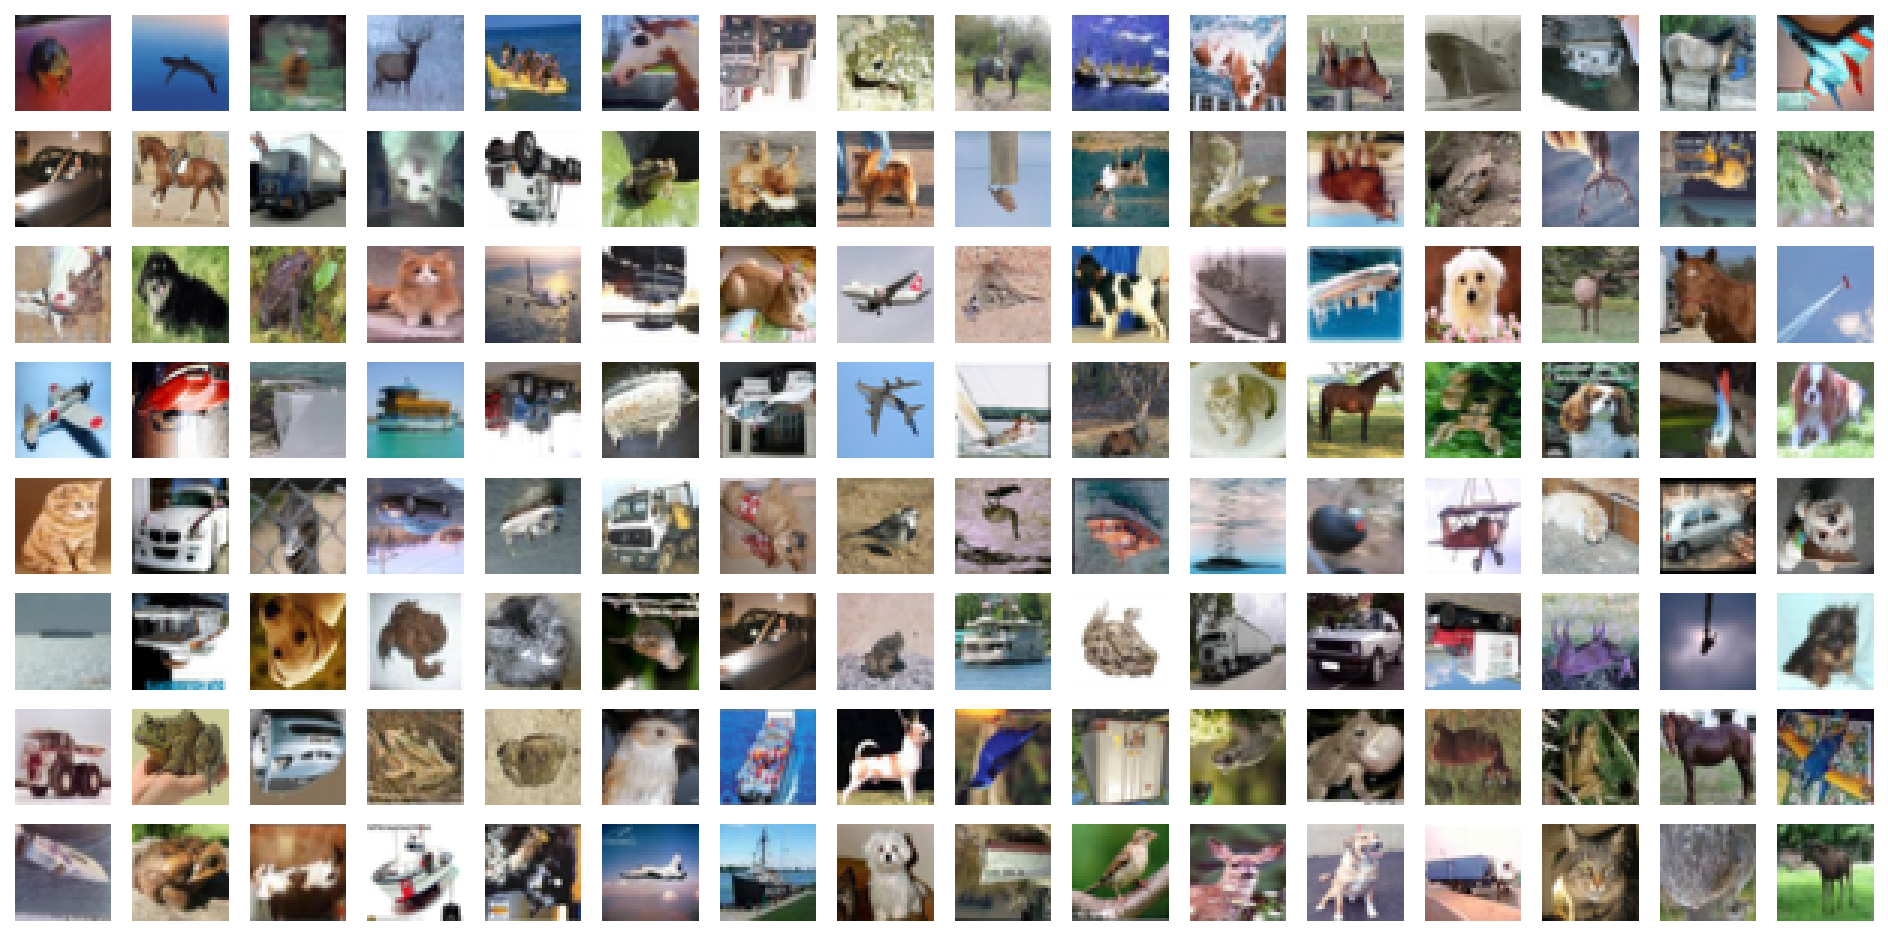
\includegraphics[width=\textwidth]{figures/cifar10_random_grid_view.pdf}
\caption{待写}
\label{fig:cifar10_random_grid_view}
\end{figure}


